\documentclass[a4paper,12pt]{article}
\usepackage{graphicx}
\graphicspath{{.}}

\usepackage{calc}
\setlength\textwidth{7in}
\setlength\textheight{10in}
\setlength\oddsidemargin{(\paperwidth-\textwidth)/2 - 1in}
\setlength\topmargin{(\paperheight-\textheight
	-\headheight-\headsep-\footskip)/2 - 1in}

\begin{document}

	
	\title{Tema Curs 7 Baze de Date}
	\author{Moroianu Theodor (135)}
	\date{\today}
	\maketitle

	\section{}
		\textit{Pe diagrama ce modelează (parțial) activitățile de închiriere ale unei agenții imobiliare, aflați
		numele chiriașilor care au vizionat toate proprietățile de închiriat avand un tarif > 1000 ale
		filialei având id-ul 15. }\\
		\newline
		\textbf{prop = SELECT(proprietate\_inchiriat, filiala=15, chirie$<$1000)\\
		prop\_id = PROJECT(prop, id)\\
		viz = PROJECT(Vizioneaza, id\_chirias, id\_proprietate)\\
		ids = DIVIDE(viz, prop\_id)\\
		Answer = PROJECT(SELECT(chirias, id in ids), nume, prenume)\\
		}
	
	\section{}
		\textit{Pentru problema 1 este propus arborele algebric din fisierul ex\_1\_optimizare.pdf.\\
		Se cer arborele algebric optimizat și expresia algebrică corespunzătoare acestuia.}\\
		\newline
		\textbf{Expresia algebrica a arborelui optimizat este:\\
		considerati = PROJECT(SELECT(salariat, salariu $>$ a), id\_salariat)\\
		prosti1 = UNION(PROJECT(publicatie, id\_salariat), PROJECT(capitol, id\_salariat))\\
		prosti2 = UNION(prosti1, PROJECT(SEMI-JON(realizeaza, frame), id\_salariat))\\		
		good\_ids = DIFFERENCE(considerati, prosti2)\\
		answer = semi-join(salariat, good\_id)}
		
		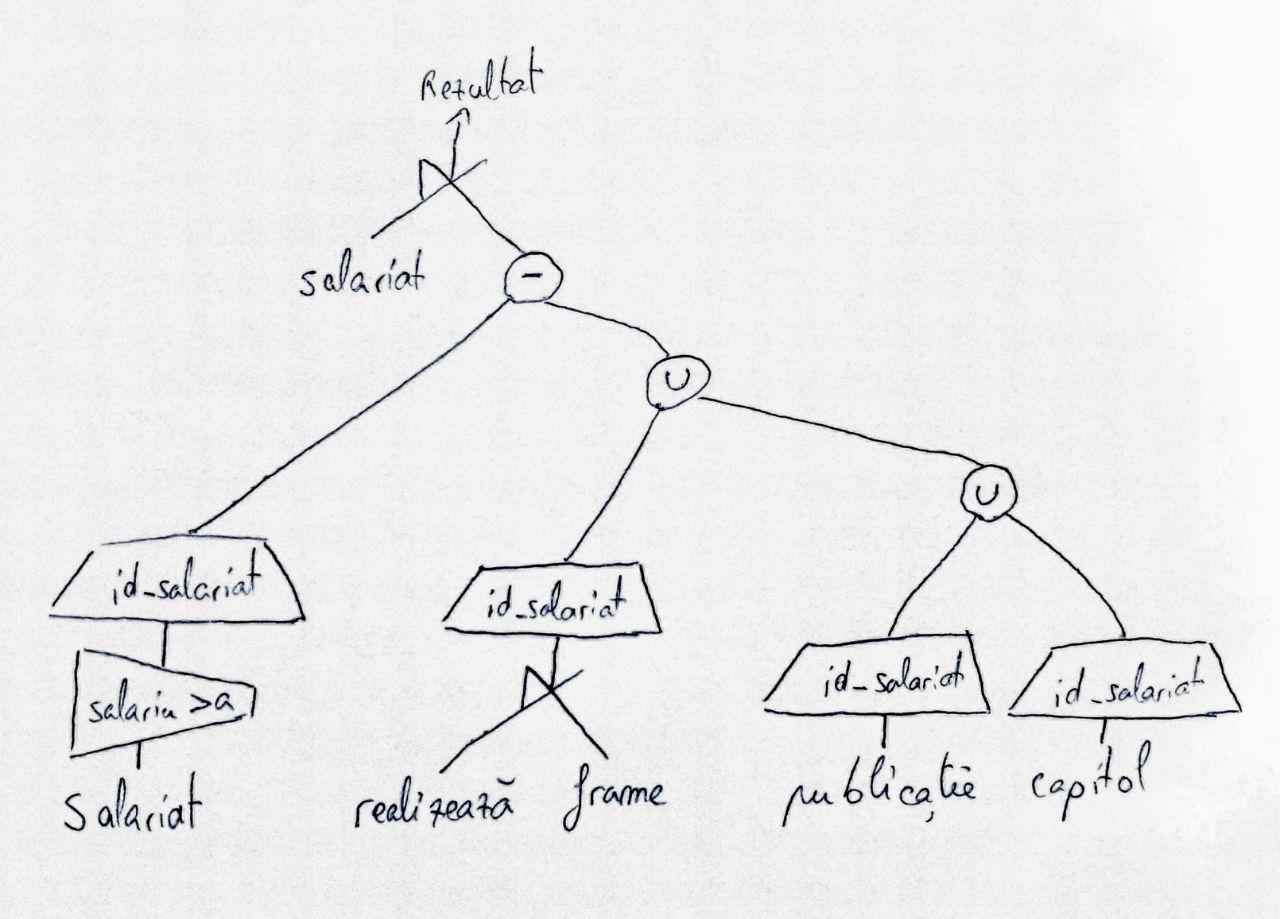
\includegraphics[scale=0.3]{ex_2_tree.jpg}
		
	
	\section{}
		\textit{Problema 2 a fost expusă la curs: am lucrat toate cele 4 variante de reprezentare a unei soluții și am comentat transformările care pot fi făcute asupra arborelui algebric pentru a-l optimiza.\\
		Se cer arborele algebric optimizat și expresia algebrică corespunzătoare acestuia.\\}
		\newline
		\textbf{Expresia algebrica optimizata este:\\
		case = SELECT(objectiv, desc="casa\_vac" OR desc="cabana")\\
		case\_selected = PROJECT(case, cod\_obiectiv)\\
		lucrari = SELECT(lucrare, tip='spec')\\
		X = SEMI-JOIN(lucrari, case\_selected)\\
		sub\_antr = PROJECT(subantreprenori, cod\_contractant, nume)\\
		answer = SEMI-JOIN(sub\_antr, X)\\}	
		
		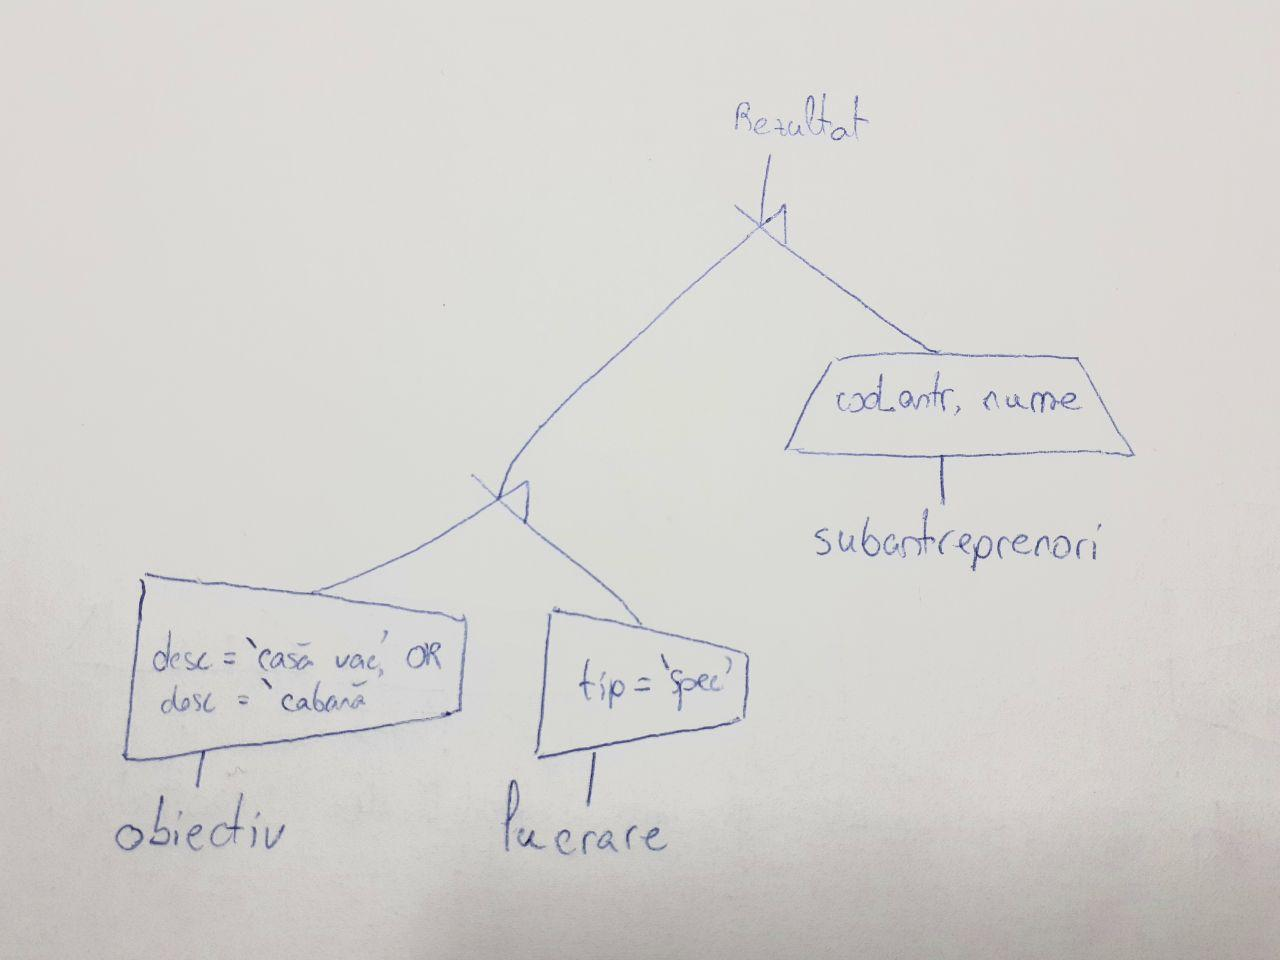
\includegraphics[scale=0.3]{ex_3_tree.jpg}
		
		\newpage
		
	\section{}
		\textit{Problema 3 a fost lucrată parțial la curs: am obținut expresia algebrică Rezultat pe baza unor relații intermediare, apoi am aplicat proprietățile P4, P5 și P3 și am obținut expresia echivalentă Rezultat\_optimizat. Să se reprezinte arborii algebrici corespunzători acestor două expresii algebrice.}\\
		
		\textbf{Arbore ne-optimizat:\\}
		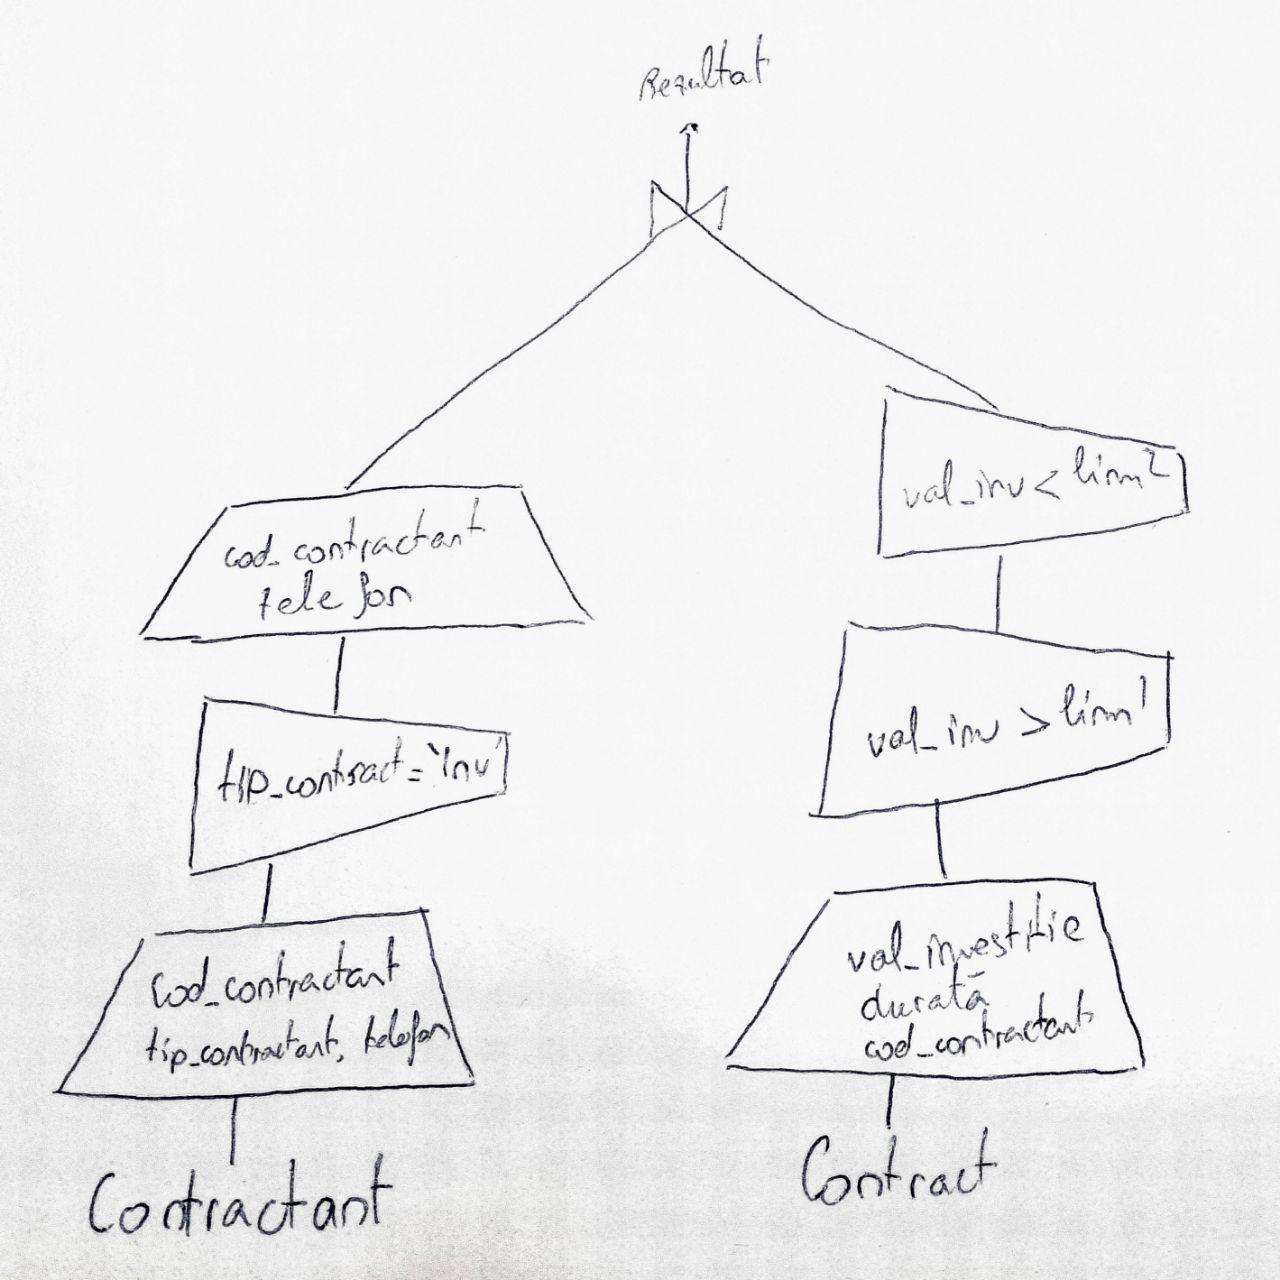
\includegraphics[scale=0.3]{ex_4_tree1.jpg}\\
		\newline
		\textbf{Arbore optimizat:\\}
		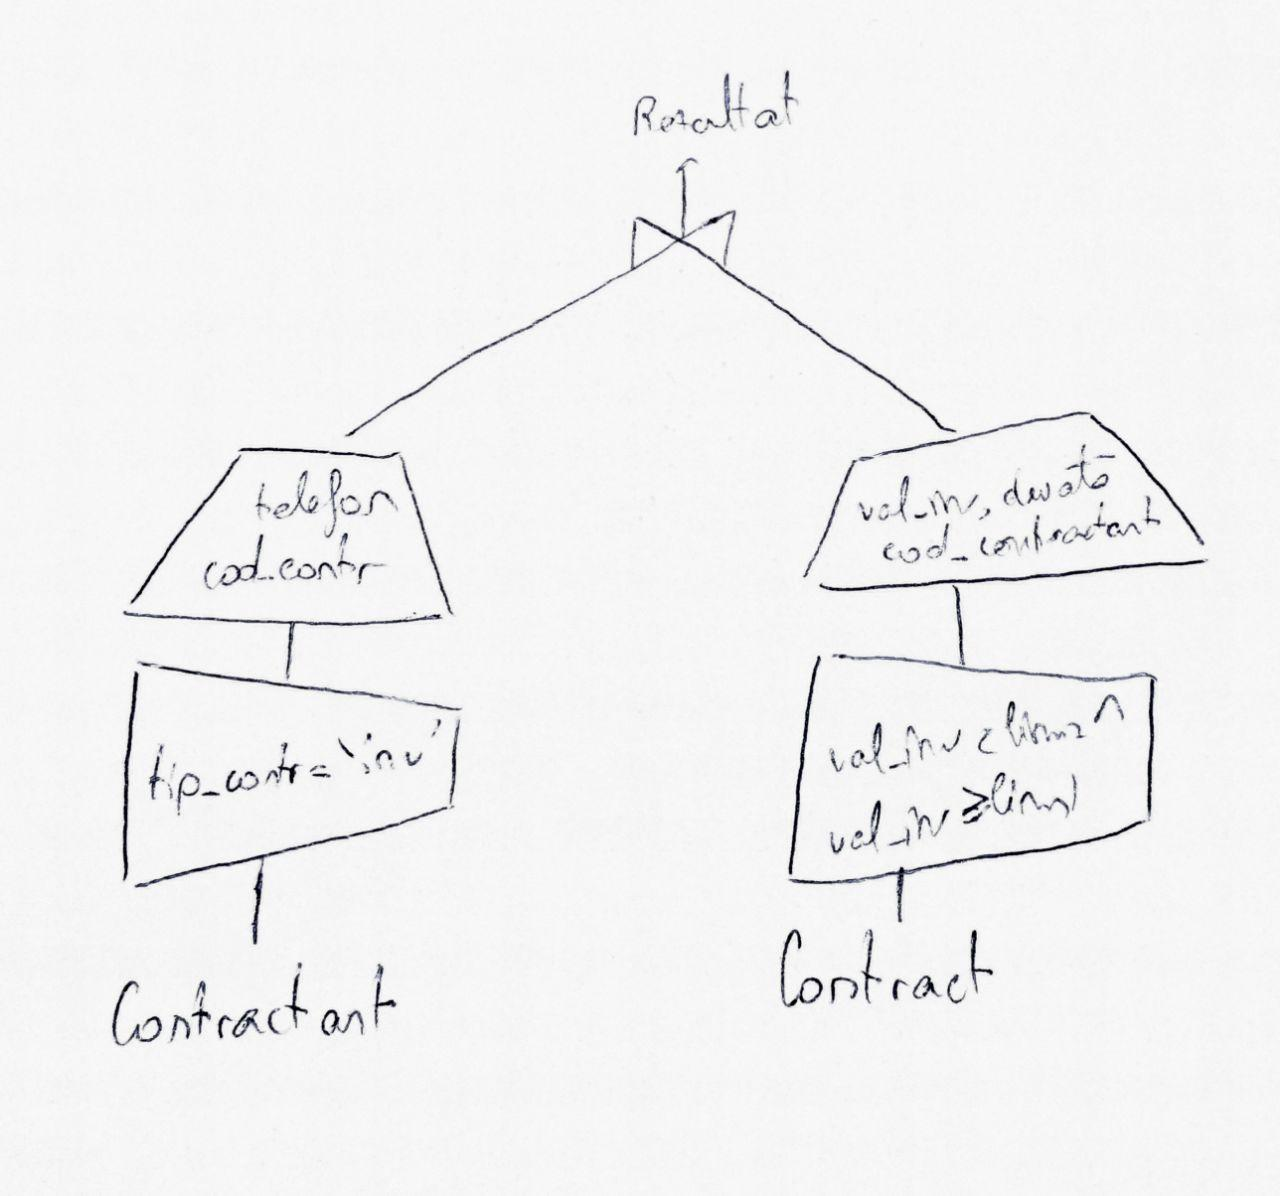
\includegraphics[scale=0.3]{ex_4_tree2.jpg}
		
		\newpage
		
	\section{}
		\textit{Pentru problema 4 este propus arborele algebric din fișierul ex\_4\_optimizare.pdf. Se cere arborele algebric optimizat.}\\
		\newline
		
		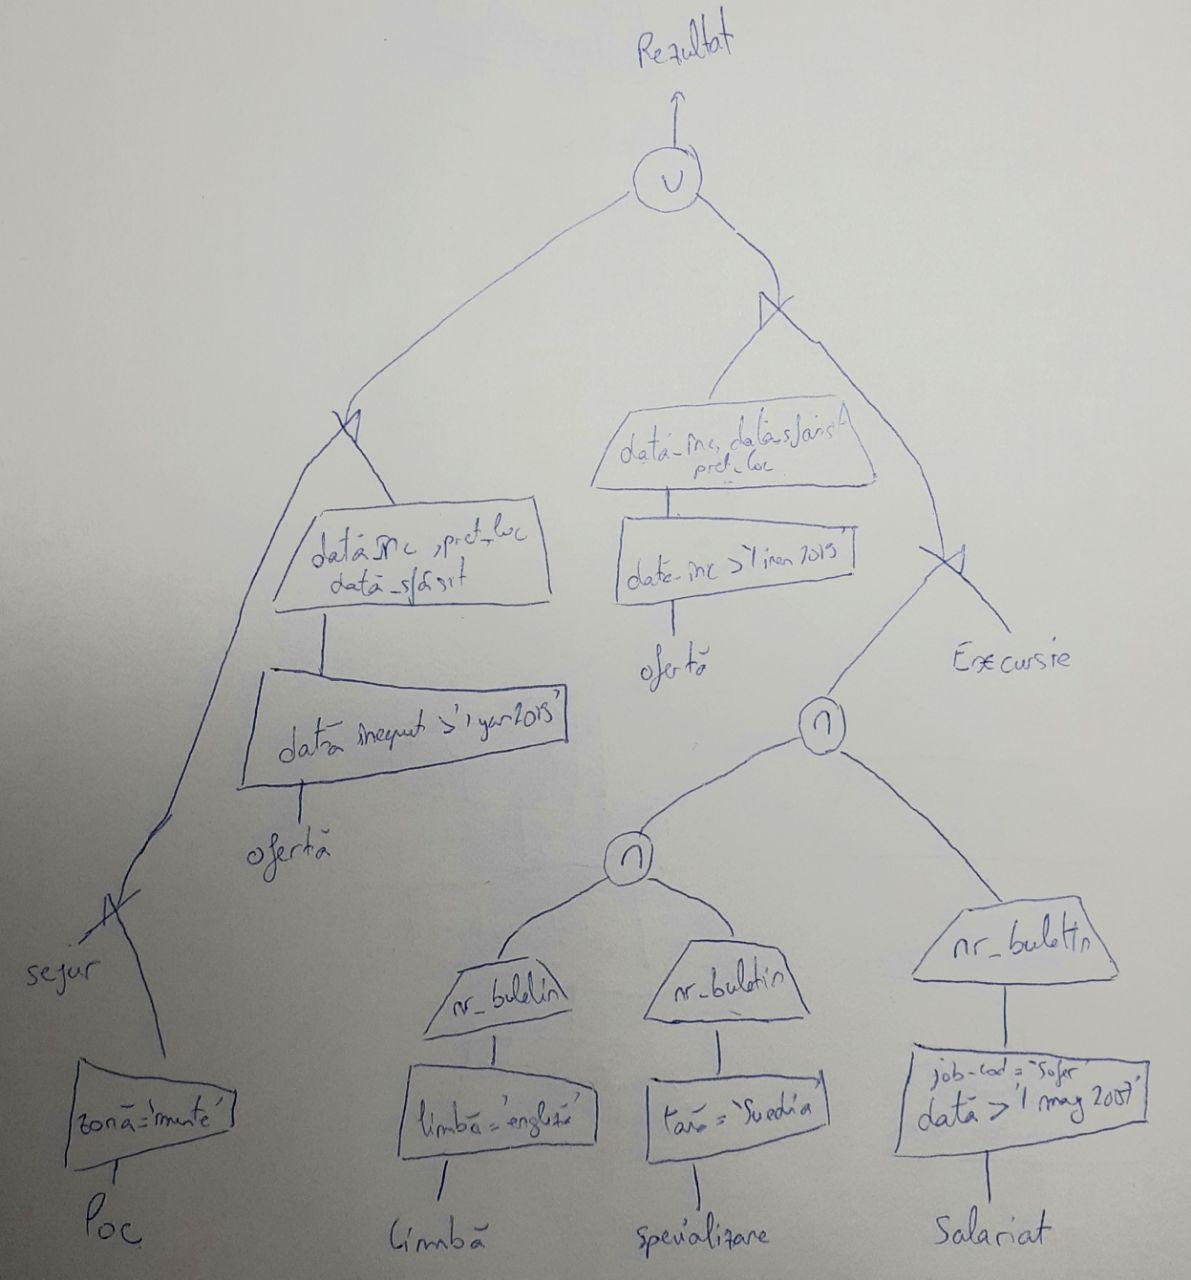
\includegraphics[scale=0.5]{ex_5_tree.jpg}
	
	
\end{document}















